\chapter{\ifproject%
\ifcpe โครงสร้างและขั้นตอนการทำงาน\else Project Structure and Methodology\fi
\else%
\ifcpe โครงสร้างของโครงงาน\else Project Structure\fi
\fi
}

ในบทนี้จะกล่าวถึงหลักการ และการออกแบบระบบ

\makeatletter

% \renewcommand\section{\@startsection {section}{1}{\z@}%
%                                    {13.5ex \@plus -1ex \@minus -.2ex}%
%                                    {2.3ex \@plus.2ex}%
%                                    {\normalfont\large\bfseries}}

\makeatother
%\vspace{2ex}
% \titleformat{\section}{\normalfont\bfseries}{\thesection}{1em}{}
% \titlespacing*{\section}{0pt}{10ex}{0pt}

\section{แผนการทำงาน}
\quad ใช้รูปแบบ software development models เป็นรูปแบบ scrum โดยแบ่งการทำงานเป็นรอบ 
โดยที่แต่ละรอบการทำงานมีระยะเวลา 1 สัปดาห์ในช่วงท้ายของแต่ละสัปดาห์จะมีการตรวจสอบความคืบหน้าของการดำเนินงานในส่วนต่าง ๆ 
และ ทุก ๆ ท้ายของรอบการทำงานจะมีการประชุมทบทวนแผนงานที่จะทำสำหรับรอบถัดไปร่วมกันเพื่อยืนยันแผนการดำเนินงานหากมีการเปลี่ยนแปลงเกิดขึ้น 
รวมถึงสรุปข้อผิดพลาดจากการทำงานในรอบนี้ด้วย
\section{การทำงานของระบบ}
\begin{figure}
\begin{center}
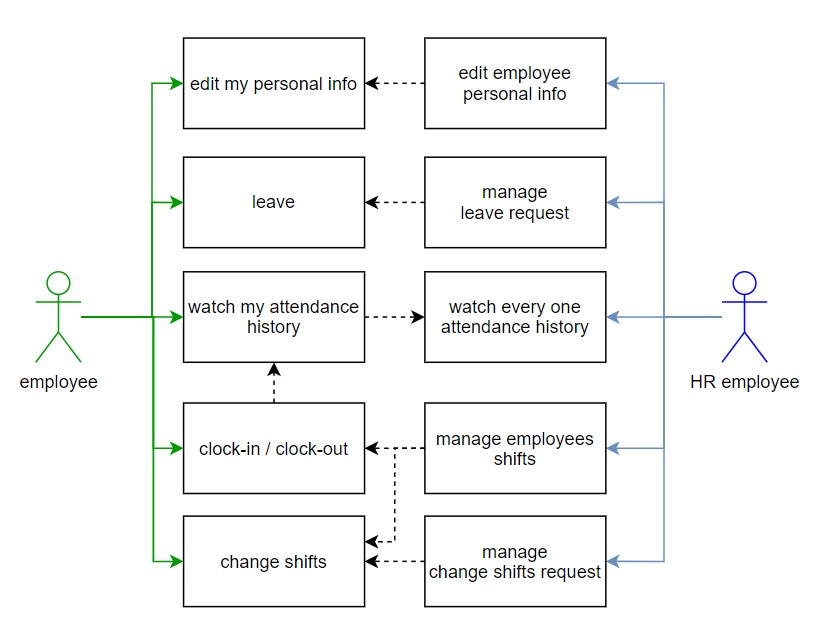
\includegraphics[width=14cm,keepaspectratio]{./images/penhwang_er_diagram_2.jpg}
\end{center}
\caption[Poem]{แสดง use case diagram ซึ่งแสดงให้เห็นกลุ่มผู้ใช้งานทั้ง 2 กลุ่มประกอบด้วย พนักงานทั่วไป (employee) และ พนักงาน hr (human resources employee)
\end{figure}

\begin{figure}
\begin{center}
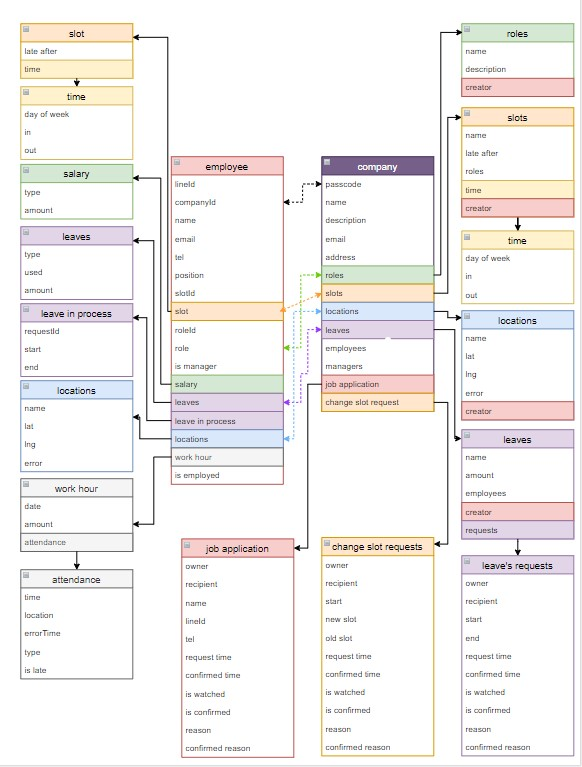
\includegraphics[width=14cm,keepaspectratio]{./images/penhwang_db_schema.jpg}
\end{center}
\caption[Poem]{แสดง E-R diagram (Entity-Relationship diagram) ซึ่งแสดงรายละเอียดของข้อมูลของแต่ละ entity ประกอบด้วย พนักงาน บริษัท และ คำขอ}
\end{figure}

\begin{figure}
\begin{center}
\includegraphics[width=14cm,keepaspectratio]{./images/structure.jpg}
\end{center}
\caption[Poem]{
  แสดงโครงสร้างของระบบ ซึ่งแบ่งเป็น 2 ส่วนใหญ่ ๆ คือ 
  front-end ประกอบด้วย LINE application (LINE bot) และ Nuxt.js 
  และ back-end (Google firebase) ซึ่งประกอบด้วย firebase cloud functions และ firebase firestore 
  โดย มี Google dialogflow ขั้นกลางระหว่าง LINE application และ firebase เพื่อทำหน้าที่แปลความหมายข้อความ
}
\end{figure}